% --- ETUDE DE CAS ---
\newpage
\section*{Étude de cas~: Résilience}
\addcontentsline{toc}{section}{Étude de cas~: Résilience}

\section*{AAV}
\addcontentsline{toc}{section}{AAV}
\begin{itemize}
	\item [3] Inventorier les différents composants du Système d'Information
	\item [3] Préparer des scripts PowerShell
	\item [3] Préparer des scripts sous Linux
	\item [5] Proposer une politique de sauvegarde au regard des besoins métiers
	\item [3] Pratiquer des outils de sauvegarde
	\item [2] Différencier les notions relatives au Plan de Continuité d'Activité
	\item [2] Différencier les types de sauvegarde
	\item [2] Expliquer l'intérêt d'externaliser certaines sauvegardes
	\item [2] Expliquer l'intérêt des contrats de maintenance au regard d'un PRA
	\item [4] Anticiper un Plan de Reprise d'Activité en partant du métier
	\item [5] Réorganiser la sécurité d'une infrastructure
\end{itemize}

\subsection*{Mots clés}
\phantomsection
\addcontentsline{toc}{subsection}{Mots clés}
\begin{itemize}
	\item RTO
	\item RPO
	\item Règle des 3-2-1
	\item NAS
	\item SLA
	\item RAID 10
	\item PRI
	\item PCI
	\item Plan de sauvegarde
	\item Résilience
	\item Souverainété
	\item Archivage
	\item Incrémentale
\end{itemize}

\subsection*{Contexte}
\phantomsection
\addcontentsline{toc}{subsection}{Contexte}
\noindent DDC ont été vicitime d'un rançongiciel qui a chiffré une partie de leurs données. L'entreprise souhaite mettre en place un plan de sauvegarde automatique plus robuste afin de garantir la résilience de son système d'information.

\subsection*{Problématique}
\phantomsection
\addcontentsline{toc}{subsection}{Problématique}
\noindent Comment concevoir et implémenter une architecture de sauvegarde résiliente et souveraine (règle 3-2-1) garantissant la continuité d'activité face aux menaces actuelles ?

\subsection*{Contraintes}
\phantomsection
\addcontentsline{toc}{subsection}{Contraintes}
\begin{itemize}
	\item Infrastructure existante à prendre en compte
	\item Technologie actuelles
	\item Règle imposé
	\item Cloud
	\item RTO / RPO
	\item Plan de sauvegarde actuel
\end{itemize}

\subsection*{Généralisation}
\phantomsection
\addcontentsline{toc}{subsection}{Généralisation}
\begin{itemize}
	\item Sécurisation
	\item Gestion des risques
\end{itemize}

\subsection*{Livrables}
\phantomsection
\addcontentsline{toc}{subsection}{Livrables}
\begin{itemize}
	\item Nouveau plan de sauvegarde
	\item Scripts de sauvegarde automatisée Powershell
	\item Nouvelle Architecture
	\item Rapport
\end{itemize}

\subsection*{Pistes de solutions}
\phantomsection
\addcontentsline{toc}{subsection}{Pistes de solutions}
\begin{itemize}
	\item SLA
	\item Augmenter le nombre de sauvegardes
\end{itemize}

\subsection*{Plan d'actions}
\phantomsection
\addcontentsline{toc}{subsection}{Plan d'actions}
\begin{itemize}
	\item Se renseigner sur les SLA
	\item Se renseigner sur les plan de sauvegarde
	\item Étudier les règles 3-2-1
	\item Se renseigner sur les rançongiciels
	\item Analyser l'infrastructure actuelle
	\item Proposer une nouvelle architecture
	\item Rédiger des scripts de sauvegarde automatisée
	\item Mettre en place un nouveau plan de sauvegarde
	\item Rédiger un rapport
\end{itemize}

\newpage
\section*{Démarche~: Résilience}
\addcontentsline{toc}{section}{Démarche~: Résilience}


\subsection*{Définition~: Mots clés}
\phantomsection
\addcontentsline{toc}{subsection}{Définition: Mots clés}


\noindent \textbf{RTO (Recovery Time Objective)}:
Le RTO est le délai maximal acceptable pour restaurer un service après une interruption. Il se définit en fonction du métier (ex. : quelques minutes pour des services critiques, heures pour des services secondaires, jours pour des services non critiques). Définir le RTO implique de planifier les actions, ressources et tests nécessaires pour atteindre cet objectif (procédures de restauration, environnements de secours, automatisation).

\vspace{0.5cm}

\noindent \textbf{RPO (Recovery Point Objective)}:
Le RPO est la quantité maximale de données qu'une organisation peut se permettre de perdre, exprimée en temps (ex. : 0s, 15 min, 24 h). Les stratégies influençant le RPO : fréquence des sauvegardes, réplication synchrone/asynchrone, journaux de transactions. Plus le RPO est court, plus le coût et la complexité augmentent.

\vspace{0.5cm}

\begin{center}
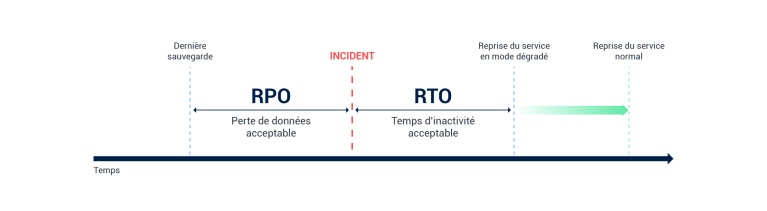
\includegraphics[width=1\textwidth]{contents/img/RTO_RPO.png}
\end{center}

\newpage
\noindent \textbf{Règle des 3-2-1 (et variantes)}:
\noindent La règle de sauvegarde 3-2-1 est une stratégie de protection des données qui consiste à conserver trois copies des données, sur deux supports différents, et à en conserver une copie hors site. Elle offre aux entreprises plusieurs niveaux de redondance : même en cas de défaillance d'un support de stockage, les autres restent disponibles.

\vspace{0.5cm}

\noindent Le principe fondamental de cette méthode de protection des données est le suivant~:

\begin{center}
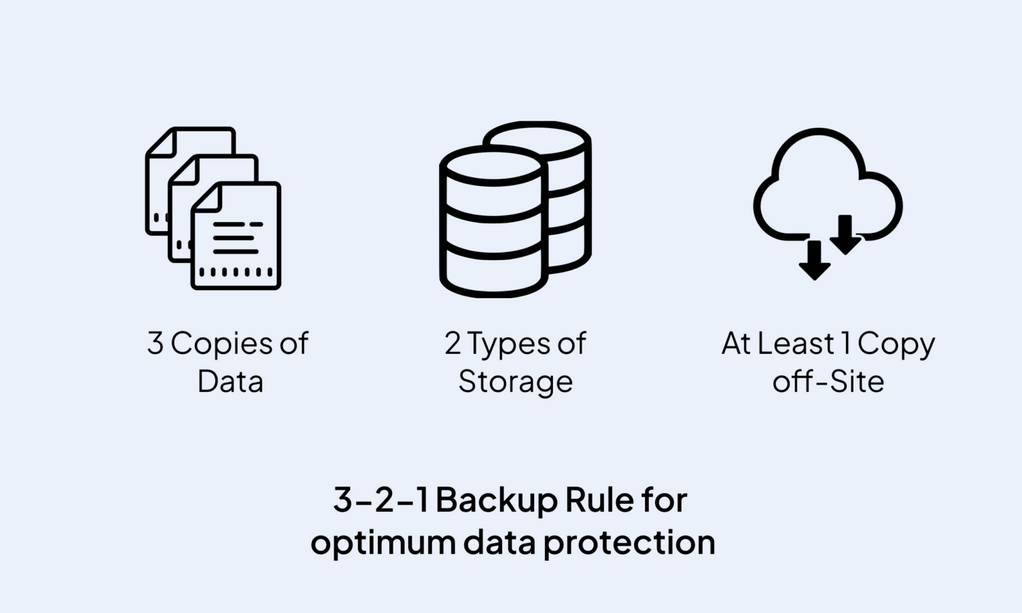
\includegraphics[width=0.7\textwidth]{contents/img/regle321.png}
\end{center}

\vspace{0.5cm}

\begin{itemize}
	\item \textbf{3 copies de données}:
	Ce processus de sauvegarde nécessite de conserver au moins trois copies de vos données. Cela comprend :
	\begin{itemize}
		\item \textbf{Une copie primaire}: Ce sont vos données de production actives et fonctionnelles.	
		\item \textbf{Deux copies de données}: La conservation de plusieurs copies réduit le risque de perte totale de données si la copie principale est endommagée ou corrompue.
	\end{itemize}

	\item \textbf{2 supports de stockage différents}:
	Le stockage des documents commerciaux sur deux supports de stockage différents réduit le risque de défaillance simultanée des deux copies en raison du même problème. Par exemple :
	\begin{itemize}
		\item \textbf{Stockage local}: les périphériques tels que les disques durs, les stockages en réseau (NAS) ou les réseaux de stockage (SAN) offrent un accès rapide aux enregistrements, mais sont sujets à des dommages physiques.	
		\item \textbf{Carte multimédia externe}: Les clés USB, les DVD ou les bandes magnétiques constituent des supports de stockage portables, mais peuvent se dégrader avec le temps.
		\item \textbf{Stockage en ligne}: Les fournisseurs de services cloud proposent un stockage d'objets fiable, mais peuvent soulever des inquiétudes concernant les accès non autorisés
	\end{itemize}

	\newpage

	\item \textbf{1 sauvegarde hors site}:
	Enfin, vous devriez conserver au moins une copie hors site afin de la protéger des risques physiques tels qu'un incendie, une inondation ou un vol de données. La sauvegarde hors site comprend souvent :
	\begin{itemize}
		\item \textbf{Solutions de sauvegarde en nuage} pour plus de commodité et d'évolutivité.
		\item \textbf{Centres de données distants} comme environnements de haute sécurité pour les données critiques sensibles.
		\item \textbf{Stockage de bandes dans des installations sécurisées hors site} pour la conservation des données à long terme.
	\end{itemize}
\end{itemize}

\noindent L'intérêt de la règle de sauvegarde 3-2-1 réside dans sa simplicité et son adaptabilité, des facteurs qui lui ont permis de rester pertinente malgré l'évolution des technologies. Que votre organisation utilise une infrastructure sur site ou un stockage entièrement basé sur le cloud, vous pouvez personnaliser cette stratégie de sauvegarde pour l'adapter à vos besoins informatiques actuels.

\vspace{0.5cm}

\noindent \textbf{NAS (Network Attached Storage)}:
Dispositif de stockage accessible sur le réseau pour fichiers partagés. Avantages : simplicité, consolidation, accès multi-utilisateurs. Limites : performances réseau, sécurité (authentification, ACL), sauvegarde dédiée (snapshots + copies vers stockage externe). Cas d'usage : stockage utilisateur, répertoires partagés, sauvegarde centralisée de fichiers.

\vspace{0.5cm}

\noindent \textbf{SLA (Service Level Agreement)}:
Contrat définissant les niveaux de service (disponibilité en \%, RTO/RPO, temps de réponse, support). Contenu typique : métriques mesurables, pénalités, fenêtres de maintenance, procédures d'escalade. Vérifier clause de localisation des données et obligations en cas d'incident.

\vspace{0.5cm}

\noindent \textbf{RAID}:
RAID (Redundant Array of Independent Disks) est une technique combinant plusieurs disques physiques pour améliorer les performances, la disponibilité et/ou la capacité. Les données peuvent être réparties (striping), dupliquées (mirroring) et/ou protégées par des informations de parité. Objectifs : augmenter les IOPS/débit, tolérance de panne et capacité effective. Attention : le RAID protège contre la défaillance matérielle d'un disque, mais n'est pas une sauvegarde (ne remplace pas les copies hors site, snapshots immuables ni la rétention).

\begin{itemize}
	\item \textbf{RAID 0 (striping)} : répartition des données sur plusieurs disques pour améliorer les performances. Aucun redondance — perte d'un disque = perte de données. Minimum 2 disques.
	\item \textbf{RAID 1 (mirroring)} : duplication exacte des données sur au moins 2 disques. Très tolérant (une copie de secours), capacité utile = 50\% du total, bonnes performances lecture.
	\item \textbf{RAID 5 (striping + parité simple)} : striping avec parité distribué. Tolère la perte d'un disque, bon compromis capacité/perf. Minimum 3 disques. Rebuilds longs et risques d'URE pendant la reconstruction.
	\item \textbf{RAID 6 (double parité)} : similaire au RAID5 mais avec parité double, tolère deux pannes simultanées. Plus sûr pour grands ensembles de disques, overhead de capacité plus élevé. Minimum 4 disques.
	\item \textbf{RAID 10 (1+0)} : combinaison de mirroring et de striping (miroirs groupés puis stripés). Excellente tolérance et performance I/O, mais coût en capacité élevé (minimum 4 disques).
	\begin{center}
		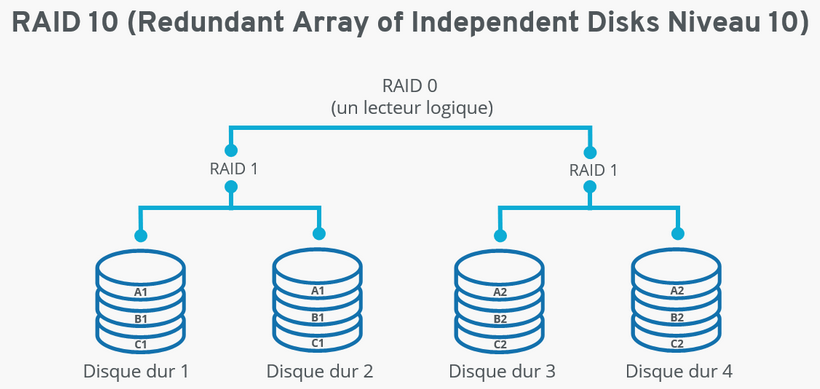
\includegraphics[width=0.7\textwidth]{contents/img/raid10.png}
	\end{center}
	\item \textbf{RAID 01 (0+1)} : striping puis mirroring — moins courant et généralement moins résilient que RAID10.
	\item \textbf{RAID 50 / RAID 60} : striping de plusieurs ensembles RAID5/RAID6 pour combiner capacité, performance et meilleure tolérance globale (utile sur grandes baies).
	\item \textbf{RAID-Z / RAID-Z2 (ZFS)} : variantes orientées ZFS semblables à RAID5/6 avec gestion intégrée d'intégrité (checksums, scrubbing) et meilleures garanties contre la corruption silencieuse.
	\item \textbf{JBOD / Spanning} : juxtaposition de disques pour augmenter la capacité sans striping ni redondance — pas de tolérance de panne.
\end{itemize}

Remarques pratiques : prévoir un disque hot-spare, contrôleur fiable (BBU/cache), surveillance S.M.A.R.T., scrubbing régulier et plans de restauration. Enfin, rappeler que RAID n'est pas une stratégie de sauvegarde : conserver des copies hors site, snapshots immuables et politique de rétention.


\vspace{0.5cm}

\noindent \textbf{PRI / PRA (Plan de Reprise d'Activité)}:
Document opérationnel décrivant comment restaurer les fonctions critiques après sinistre (responsabilités, procédures, environnements de secours, ordre de restauration, communications). Doit inclure tests périodiques, scénarios, dépendances métiers et priorisation des services.

\vspace{0.5cm}

\noindent \textbf{PCI / PCA (Plan de Continuité d'Activité)}:
Plan visant à maintenir les opérations critiques pendant et après une perturbation (processus temporaires, équipes de secours, sites alternatifs). Se distingue du PRA qui se concentre sur la remise en service complète ; les deux sont complémentaires.

\vspace{0.5cm}

\noindent \textbf{Plan de sauvegarde}:
Stratégie définissant quoi, quand, où et comment sauvegarder : inventaire des données, politique de fréquence (full/incrémentale/ différentielle), rétention, chiffrement, rotation des médias, stockage hors site, procédures de restauration et tests réguliers. Inclure des métriques (fenêtres de sauvegarde, taux d'échec acceptable) et l'automatisation des vérifications (intégrité, restaurations partielles).

\vspace{0.5cm}

\noindent \textbf{Résilience}:
Capacité d'un système à résister, détecter et récupérer rapidement des perturbations. Principes : redondance, diversité des technologies et lieux, isolation des défaillances, détection/monitoring, automatisation des basculements, tests réguliers et amélioration continue. Mesurer via disponibilité, MTTR et MTBF.

\vspace{0.5cm}

\noindent \textbf{Souveraineté (des données)}:
Contrôle de l'hébergement, du traitement et de la juridiction des données. Mesures : choix de régions/centres de données, chiffrement avec clés propriétaires, clauses contractuelles, audits et certification des fournisseurs. Attention aux transferts transfrontaliers et obligations réglementaires.

\vspace{0.5cm}

\noindent \textbf{Archivage}:
Conservation à long terme de données pour conformité ou valeur historique. Comprend politiques de conservation, formats pérennes, migration planifiée, indexation et capacités de recherche. Solutions : stockage WORM, bande, stockage objet à long terme avec cycle de migration.

\vspace{0.5cm}

\noindent \textbf{Incrémentale (sauvegarde)}:
Stratégie où seules les modifications depuis la dernière sauvegarde sont copiées. Types : incrémentale classique (chaînage), différentielle (depuis le dernier full), incrémentale cumulative, « incremental-forever » + synthetic full. Avantages : gain de temps et espace ; inconvénients : restauration potentiellement plus lente si chaîne longue. Bonnes pratiques : checkpoints, synthetic full réguliers, vérification d'intégrité, documentation des chaînes de sauvegarde.

\newpage

\section*{Corbeille d'Excercice}
\addcontentsline{toc}{section}{Corbeille d'Excercice}
\noindent Cette corbeille va utiliser les VM installées dans la séquence de préparation, Bash et PowerShell.

\noindent L’objectif est de progresser dans l’utilisation PowerShell, de Bash et de prendre en main les outils de sauvegardes Windows et Linux.

\noindent Il a souvent été constaté que les services informatiques ont du mal à répondre aux questions suivantes :

\begin{itemize}
	\item Vérifiez-vous régulièrement le bon déroulement /réalisation des sauvegardes ?
	\item Vos sauvegardes sont-elles testées et validées ?
	\item Avez-vous déjà effectué une restauration à partir des sauvegardes réalisées suite à un incident/crash d'un ou plusieurs serveurs ?
\end{itemize}

\noindent Il faut savoir que le Reporting des sauvegardes est un élément critique et important pour toute direction
informatique.

\noindent Réaliser des sauvegardes c'est bien, mais savoir les utiliser en cas de problème est OBLIGATOIRE.

\noindent Quand vous réalisez vos sauvegardes, vous devez vous assurer que celles-ci ont bien été effectuées, car il arrive parfois que des sauvegardes échouent suite à une saturation d'espace disque (sur l'emplacement de sauvegarde) ou simplement à cause d'un problème de performance.

\subsection*{Matériel nécessaire}
\phantomsection
\addcontentsline{toc}{subsection}{Matériel nécessaire}
\noindent Vous avez besoin d'une VM Windows Server et d'une VM Ubuntu Server.

\subsection*{Rappels~: PowerShell et Bash}
\phantomsection
\addcontentsline{toc}{subsection}{Rappels~: PowerShell et Bash}
\noindent PowerShell est un shell de ligne de commande et un langage de script développé par Microsoft, principalement utilisé pour l'automatisation des tâches d'administration système sur les systèmes Windows. Il permet aux administrateurs de gérer les configurations, d'automatiser les processus et d'interagir avec divers services et applications Windows.

\noindent Bash (Bourne Again SHell) est un shell de ligne de commande et un langage de script largement utilisé dans les systèmes d'exploitation Unix et Linux. Il permet aux utilisateurs d'exécuter des commandes, d'automatiser des tâches et de gérer les configurations système à travers des scripts.

\newpage

Question~: Quelle version de PowerShell utilise Windows Server 2022 et Windows 10 ?

\noindent Réponse~: Windows Server 2022 et Windows 10 utilisent PowerShell 5.1 par défaut, mais PowerShell 7.x (PowerShell Core) peut également être installé en tant que version multiplateforme plus récente.

\vspace{0.5cm}

Question~: Qu'est ce qu'un script Shell ?

\noindent Réponse~: Un script Shell est un fichier texte contenant une série de commandes écrites dans un langage de script spécifique (comme Bash ou PowerShell) qui peuvent être exécutées par un interpréteur de commandes pour automatiser des tâches système.

\vspace{0.5cm}

Question~: Qu'est-ce Bash et comment connaitre sa version ?

\noindent Réponse~: Bash (Bourne Again SHell) est un shell de ligne de commande et un langage de script utilisé principalement dans les systèmes Unix et Linux. Pour connaître la version de Bash installée sur votre système, vous pouvez exécuter la commande suivante dans le terminal~:
\begin{verbatim}
bash --version
\end{verbatim}

\vspace{0.5cm}

Questions~: Comment rendre un script Shell exécutable sur votre serveur?

\noindent Réponse~: Pour rendre un script Shell exécutable sur votre serveur, vous devez modifier les permissions du fichier en utilisant la commande chmod. Par exemple, pour rendre un script nommé script.sh exécutable, vous pouvez utiliser la commande suivante~:
\begin{verbatim}
chmod +x script.sh
\end{verbatim}

\vspace{0.5cm}

Questions~: Que font les commandes suivantes : man, cd, ls, pwd, mkdir, rm, mv, cp, file, echo, cat, head, tail, touch, history, cal, grep?

\noindent Réponse~:
\begin{itemize}
	\item man : Affiche le manuel d'une commande.
	\item cd : Change le répertoire courant.
	\item ls : Liste les fichiers et répertoires dans le répertoire courant.
	\item pwd : Affiche le chemin du répertoire courant.
	\item mkdir : Crée un nouveau répertoire.
	\item rm : Supprime des fichiers ou répertoires.
	\item mv : Déplace ou renomme des fichiers ou répertoires.
	\item cp : Copie des fichiers ou répertoires.
	\item file : Détermine le type d'un fichier.
	\item echo : Affiche une ligne de texte ou une variable.
	\item cat : Affiche le contenu d'un fichier.
	\item head : Affiche les premières lignes d'un fichier.
	\item tail : Affiche les dernières lignes d'un fichier.
	\item touch : Crée un fichier vide ou met à jour la date de modification d'un fichier.
	\item history : Affiche l'historique des commandes exécutées.
	\item cal : Affiche un calendrier.
	\item grep : Recherche des motifs dans un fichier ou une entrée.
\end{itemize}

\subsection*{EXERCICES SCRIPTS SHELL}
\phantomsection
\addcontentsline{toc}{subsection}{EXERCICES SCRIPTS SHELL}
\noindent Voici quelques exercices pratiques.

Questions~: Comment écrire une boucle affichant les entiers divisibles par 3 entre 1 et 100 ?

\noindent Réponse~:
\begin{verbatim}
for i in {1..100}
do
  if (( i % 3 == 0 )); then
	echo $i
  fi
done
\end{verbatim}

Questions~: Comment écrire un script shell qui affiche “répertoire présent” si l’argument de la commande correspond à un répertoire qui existe ?

\noindent Réponse~:
\begin{verbatim}
#!/bin/bash
if [ -d "$1" ]; then
  echo "répertoire présent"
else
  echo "répertoire absent"
fi
\end{verbatim}

\newpage

\subsection*{Comparaison PowerShell / Bash}
\phantomsection
\addcontentsline{toc}{subsection}{Comparaison PowerShell / Bash}
\noindent Voici une comparaison entre PowerShell et Bash pour certaines tâches courantes.

\vspace{0.5cm}

\begin{center}
\begin{tabular}{|p{3.5cm}|p{5cm}|p{5cm}|}
\hline
\textbf{Caractéristique} & \textbf{PowerShell} & \textbf{Shell script (Bash, sh...)} \\
\hline
Plateforme d'origine & Windows & Unix/Linux \\
\hline
Langage & PowerShell (orienté objets .NET) & Bash / Bourne shell (texte et chaînes) \\
\hline
Fichiers script & .ps1 & .sh \\
\hline
Syntaxe & Style Cmdlet (Verbe-Nom) & Commandes classiques (ls, cat, grep, ...) \\
\hline
Manipulation des données & Orienté objet (les commandes retournent des objets riches) & Manipulation de texte (chaînes et flux uniquement) \\
\hline
\end{tabular}
\end{center}

\newpage

\section*{Analyse et résolution : Résilience}
\addcontentsline{toc}{section}{Analyse et résolution : Résilience}
	
\subsection*{Les rançongiciels : Rappel}
\phantomsection
\addcontentsline{toc}{subsection}{Les rançongiciels : Rappel}
\noindent Les rançongiciels (ransomware) sont des logiciels malveillants qui chiffrent les données d'une victime, rendant les fichiers inaccessibles jusqu'à ce qu'une rançon soit payée. Ils se propagent souvent via des courriels de phishing, des vulnérabilités logicielles ou des téléchargements malveillants. Pour se protéger contre les rançongiciels, il est crucial de maintenir des sauvegardes régulières, de mettre à jour les systèmes, d'utiliser des solutions de sécurité robustes et de sensibiliser les utilisateurs aux risques.

\subsection*{Analyse de l'existant — Infrastructure de sauvegarde actuelle}
\phantomsection
\addcontentsline{toc}{subsection}{Analyse de l'existant — Infrastructure de sauvegarde actuelle}

\noindent \textbf{Présentation synthétique} :
\begin{itemize}
	\item Topologie : deux réseaux dédiés aux sauvegardes, chacun raccordé à un NAS distinct — NAS interne (salle serveur de l’entreprise) et NAS externe (salle serveur de la technopole).
	\item Objectifs de service actuels : RTO = 24 h, RPO = 24 h (sauvegardes quotidiennes).
	\item Politique de conservation : copies internes conservées 30 jours, copies externes conservées 7 jours.
\end{itemize}

\noindent \textbf{Synthèse} :

\noindent Données et volumes (extrait) :
\begin{itemize}
	\item Topologie : NAS interne + NAS externe, sauvegardes quotidiennes (RTO/RPO = 24 h).
	\item Volumes critiques $\approx$ 2 To (clients, finances, projets). données de projet (1 To) -- total critique $\approx$ 2 To.
	\item NAS : 4×6 To en RAID6, CPU modeste, 4~GB RAM, 2×1~GbE.
\end{itemize}

\noindent Risques clés : NAS (BERRIA) :
\begin{itemize}
	\item RTO/RPO 24 h insuffisant pour données critiques.
	\item Rétention externe 7~j trop courte ; pas d'immutabilité documentée.
	\item Réseau 1~GbE = goulot pour restaurations lourdes : 4 × 6 To en RAID 6 → capacité utile approximative : (4-2)×6 = 12 To.
	\item Peu de RAM/CPU pour dédup/chiffrement/snapshots.
	\item Connectivité : 2 × 1~GbE ; ports USB 3.2.
\end{itemize}

\subsection*{Proposition d'une nouvelle architecture de sauvegarde}
\phantomsection
\addcontentsline{toc}{subsection}{Proposition d'une nouvelle architecture de sauvegarde}

\noindent \textbf{Objectifs de service cibles} :
\begin{itemize}
	\item RTO = 4 h pour données critiques, 12 h pour secondaires.
	\item RPO = 1 h pour données critiques, 6 h pour secondaires.
	\item Conservation : copies internes 90 jours, copies externes 30 jours.
\end{itemize}

\vspace{0.5cm}

\noindent \textbf{Architecture proposée} :
\begin{itemize}
	\item Remplacement NAS interne par appliance dédiée (ex. : Synology RS422+) : CPU plus puissant, 16~GB RAM, 10~GbE.
	\item Configuration RAID recommandée :
	\begin{itemize}
		\item Pour performances et tolérance de panne (IOPS, reconstructions rapides) : RAID 10 (miroir + striping) sur disques 7200~RPM ou NVMe selon budget.
		\item Alternative pour très grande capacité : RAID6 ou RAID-Z2 (double parité) en acceptant des temps de reconstruction plus longs et un impact I/O élevé pendant la reconstruction.
		\item Prévoir au minimum un disque hot-spare, contrôleur avec cache/BBU ou stockage basé sur ZFS avec scrubbing régulier et checksums pour détecter la corruption silencieuse.
		\item Rappel : le RAID n'est pas une sauvegarde. Conserver snapshots immutables et copies hors site (règle 3-2-1).
	\end{itemize}
	\item NAS externe : migration vers solution cloud souveraine (ex. : OVHcloud Object Storage) avec chiffrement côté client.
	\item Sauvegardes différentielles/incrémentales fréquentes (toutes les heures pour critiques).
	\item Implémentation de snapshots immutables sur NAS interne.
	\item Automatisation des tests de restauration mensuels.
	\item Monitoring et alerting : S.M.A.R.T., intégrité RAID, alertes réseau et tableaux de bord pour suivre l'état des rebuilds et la latence.
\end{itemize}

\vspace{0.5cm}

\noindent \textbf{Avantages attendus} :
\begin{itemize}
	\item RTO/RPO améliorés pour données critiques.
	\item Meilleure résilience contre rançongiciels (immutabilité, copies hors site).
	\item Scalabilité via stockage cloud.
	\item Automatisation des vérifications de sauvegarde.
\end{itemize}

\subsection*{Scripts de sauvegarde automatisée}
\phantomsection
\addcontentsline{toc}{subsection}{Scripts de sauvegarde automatisée}
\noindent Voici des exemples de scripts pour automatiser les sauvegardes sur Windows (PowerShell) et Linux (Bash).

\vspace{0.5cm}

\noindent \textbf{PowerShell (Windows Server)} :
\begin{verbatim}
# Script de sauvegarde PowerShell
$source = "C:\DonnéesCritiques"
$destination = "\\NASInterne\Sauvegardes\DonnéesCritiques"
$logFile = "C:\Logs\Sauvegarde.log"
$date = Get-Date -Format "yyyy-MM-dd_HH-mm-ss"
# Créer le répertoire de destination avec horodatage
$destPath = Join-Path $destination $date
New-Item -ItemType Directory -Path $destPath
# Copier les fichiers
Robocopy $source $destPath /MIR /Z /R:3 /W:5 /LOG:$logFile
# Vérifier le succès
if ($LASTEXITCODE -le 3) {
	Write-Output "Sauvegarde réussie : $date" >> $logFile
} else {
	Write-Output "Erreur de sauvegarde : $date" >> $logFile
}
\end{verbatim}

\vspace{0.5cm}

\noindent \textbf{Bash (Ubuntu Server)} :
\begin{verbatim}
#!/bin/bash
# Script de sauvegarde Bash
SOURCE="/home/ubuntu/donnees_critique"
DESTINATION="/mnt/nas_interne/sauvegardes/donnees_critique"
LOGFILE="/var/log/sauvegarde.log"
DATE=$(date +"%Y-%m-%d_%H-%M-%S")
# Créer le répertoire de destination avec horodatage
DEST_PATH="$DESTINATION/$DATE"
mkdir -p "$DEST_PATH"
# Copier les fichiers
rsync -av --delete "$SOURCE/" "$DEST_PATH/" >> "$LOGFILE" 2>&1
# Vérifier le succès
if [ $? -eq 0 ]; then
	echo "Sauvegarde réussie : $DATE" >> "$LOGFILE"
else
	echo "Erreur de sauvegarde : $DATE" >> "$LOGFILE"
fi
\end{verbatim}

\subsection*{Rapport de synthèse}
\phantomsection
\addcontentsline{toc}{subsection}{Rapport de synthèse}
\noindent \textbf{Résumé exécutif} :
Suite à l'incident de rançongiciel ayant affecté DDC, une analyse approfondie de l'infrastructure de sauvegarde actuelle a révélé plusieurs lacunes critiques, notamment des objectifs de RTO/RPO inadéquats, une rétention insuffisante des données et des limitations matérielles du NAS interne. Pour remédier à ces faiblesses, une nouvelle architecture de sauvegarde a été proposée, incluant le remplacement du NAS interne par une appliance plus performante, la migration vers une solution de stockage cloud souveraine pour les sauvegardes externes, et l'implémentation de stratégies de sauvegarde plus fréquentes et de snapshots immutables. Ces mesures visent à améliorer significativement la résilience du système d'information de DDC, en garantissant une meilleure protection contre les menaces actuelles et en assurant la continuité des activités critiques de l'entreprise.

\vspace{0.5cm}


\subsection*{Conclusion}
\phantomsection
\addcontentsline{toc}{subsection}{Conclusion}
\noindent La mise en place d'une architecture de sauvegarde résiliente et souveraine est essentielle pour garantir la continuité des activités face aux menaces croissantes telles que les rançongiciels. En adoptant des stratégies de sauvegarde robustes, en utilisant des technologies adaptées et en automatisant les processus de vérification, les organisations peuvent minimiser les risques de perte de données et assurer une reprise rapide en cas d'incident. La résilience du système d'information n'est pas seulement une question de technologie, mais aussi de planification, de formation et de vigilance continue.

\newpage

\subsection*{Capitalisation}
\phantomsection
\addcontentsline{toc}{subsection}{Capitalisation}
\noindent Cette étude de cas a permis de renforcer les compétences en analyse d'infrastructures de sauvegarde, en conception d'architectures résilientes et en automatisation des processus de sauvegarde. Les connaissances acquises sur les rançongiciels, les objectifs de RTO/RPO et les meilleures pratiques de sauvegarde seront précieuses pour la gestion future des systèmes d'information. La mise en œuvre de solutions de sauvegarde robustes contribuera à la sécurité et à la continuité des opérations, tout en sensibilisant davantage aux enjeux de la résilience informatique.

\subsection*{Ressources}
\phantomsection
\addcontentsline{toc}{subsection}{Ressources}

\begin{itemize}
	\item \textbf{RTO et RPO} : \url{https://www.ibm.com/docs/en/tsm/7.1.0?topic=concepts-recovery-time-objective-rto-recovery-point-objective-rpo}
	\item \textbf{Règle des 3-2-1} : \url{https://www.backblaze.com/blog/the-3-2-1-backup-strategy}
	\item \textbf{NAS} : \url{https://www.synology.com/en-global/knowledgebase/DSM/tutorial/Storage/What_is_NAS}
	\item \textbf{SLA} : \url{https://www.atlassian.com/fr/incident-management/service-level-agreements}
	\item \textbf{RAID 10} : \url{https://www.crucial.fr/articles/about-ssd/what-is-raid-10}
	\item \textbf{PRA et PCA} : \url{https://www.iso.org/iso-22301-business-continuity.html}
	\item \textbf{Plan de sauvegarde} : \url{https://www.veeam.com/blog/backup-strategy-best-practices.html}
	\item \textbf{Résilience} : \url{https://www.gartner.com/en/information-technology/glossary/resilience}
	\item \textbf{Souveraineté des données} : \url{https://www.dataprotectionreport.com/2020/01/data-sovereignty-and-the-cloud}
	\item \textbf{Archivage} : \url{https://www.archiving.com/what-is-data-archiving}
	\item \textbf{Sauvegarde incrémentale} : \url{https://www.backupassist.com/blog/understanding-incremental-backups}
	\item \textbf{Rançongiciels} : \url{https://www.cisa.gov/ransomware}
\end{itemize}
